\documentclass[11pt]{article}
\usepackage[margin=1in]{geometry}
\usepackage{amsmath,amssymb,amsthm}
\usepackage{graphicx}
\usepackage{tikz}
\usetikzlibrary{arrows.meta,positioning,decorations.pathmorphing,calc}
\usepackage{booktabs}
\usepackage[colorlinks=true,linkcolor=blue!50!black,citecolor=blue!50!black,urlcolor=blue!50!black]{hyperref}
\usepackage{enumitem}

\theoremstyle{plain}
\newtheorem{theorem}{Theorem}
\newtheorem{proposition}[theorem]{Proposition}
\newtheorem{lemma}[theorem]{Lemma}
\newtheorem{corollary}[theorem]{Corollary}
\theoremstyle{definition}
\newtheorem{definition}[theorem]{Definition}
\newtheorem{remark}[theorem]{Remark}
\newtheorem{exercise}{Exercise}

\newcommand{\eps}{\varepsilon}
\newcommand{\R}{\mathbb{R}}
\newcommand{\Sph}{\mathbb{S}}
\newcommand{\dd}{\,\mathrm{d}}
\newcommand{\Gam}{\Gamma}

\title{\bf A Contact--Geometric Toy Model on the Solid Cylinder:\\
Transverse Stability, Closure--Dependent Escape,\\
Degenerate Hopf Structure, and a Cosmological No--Go}

\author{Pablo Grossi\thanks{G6 LLC, Newark, NJ, USA. \texttt{ORCID: 0009-0000-6496-2186}. \emph{Byline and affiliation to be confirmed by the author.}}}

\date{\today}

\begin{document}
\maketitle

\begin{abstract}
We study the transverse dynamics near the helical periodic orbit
$\Gam=\{r=1\}$ of a dissipative flow on the contact $3$--manifold
$(\R_{>0}\times\Sph^1\times\R,\ \alpha=\dd z-r^2\dd\theta)$, in which the
transverse relaxation is modulated by a factor $1-e^{-z}$. Six results are
established, each verified both numerically (double--precision \texttt{DOP853},
\texttt{rtol}$=10^{-10}$) and, where tractable, formally (Lean~4 / Mathlib4).
(i)~The linearised transverse equation admits a closed form, and its Lyapunov
exponent $\mu=-2$ is \emph{preserved} because the $e^{-z}$ modulation is
integrable along the $z$--flow, contributing only a bounded additive
distortion. (ii)~The instantaneous contraction rate changes sign on the
\emph{neutral line} $z=0$: relaxation for $z>0$, expansion for $z<0$, with the
sub--line flow the exact time reversal of the super--line flow. (iii)~The
\emph{global} fate is closure--dependent: a cubic closure exhibits genuine
finite--time escape below an analytically characterised basin boundary
$z_0^\ast(\eps_0)$, whereas any bounded closure converges globally --- so
``where it will not converge'' is a real prediction only for super--linear
closures. (iv)~At the axis $r=0$ the flow carries a \emph{degenerate} Hopf
bifurcation whose first Lyapunov coefficient vanishes at onset, pinning the
cycle radius at $1$ rather than opening it as $\sqrt{\lambda}$.
(v)~A kinematic reading $z=\ln a$ identifies $\dot z=1$ with de~Sitter
expansion and $e^{-z}$ with the inverse scale factor; we state precisely the
three obstructions that prevent this correspondence from being promoted to a
dynamical model. (vi)~We prove a \emph{no--go}: under any contact--Hamiltonian
flow of $\alpha$ with constant rotation, the transverse rate is locked to the
derivative of the expansion rate, $c(z)=H'(z)$, whence a transverse attractor
and a de~Sitter expansion rate cannot coexist. A graded problem set with
solutions accompanies the paper.
\end{abstract}

\tableofcontents

\section{Setup and the model}\label{sec:setup}

Let $M=\{(r,\theta,z):r>0,\ \theta\in\Sph^1,\ z\in\R\}$ carry the contact
$1$--form
\begin{equation}
\alpha \;=\; \dd z - r^2\,\dd\theta .
\end{equation}
One checks $\alpha\wedge\dd\alpha = -2r\,\dd r\wedge\dd\theta\wedge\dd z\neq0$,
so $\alpha$ is contact and the Reeb field is $R=\partial_z$. Writing
$p:=r^2$ for the momentum conjugate to $\theta$, the form is the standard
Hamilton--Jacobi contact form $\alpha=\dd z-p\,\dd\theta$.

We study the flow
\begin{equation}\label{eq:model}
\dot r \;=\; f(r)\,\bigl(1-e^{-z}\bigr),\qquad
\dot\theta \;=\; 1,\qquad
\dot z \;=\; 1,
\end{equation}
where the \emph{closure} $f:\R_{>0}\to\R$ satisfies
\begin{equation}\label{eq:closure-cond}
f(1)=0,\qquad f'(1)=-2,\qquad f(r)\,(r-1)<0 \ \ (r>0,\ r\neq1).
\end{equation}
Conditions~\eqref{eq:closure-cond} make $\Gam=\{r=1\}$ a periodic orbit of
period $T^\ast=2\pi$ (a helix in $(r,\theta,z)$, since $\dot\theta=\dot z=1$),
with clean transverse eigenvalue $-2$ when the modulation saturates
($z\to+\infty$). Two canonical closures obey~\eqref{eq:closure-cond}:
\begin{equation}
f_{\mathrm{cub}}(r)=r-r^3 \quad(\text{super--linear}),\qquad
f_{\mathrm{sat}}(r)=\frac{-2(r-1)}{1+(r-1)^2}\quad(\text{bounded}).
\end{equation}
Both have $f(1)=0$, $f'(1)=-2$; they differ only in their large--$r$
behaviour, and \S\ref{sec:closure} shows that this difference alone decides
global dynamics.

\begin{figure}[t]
\centering
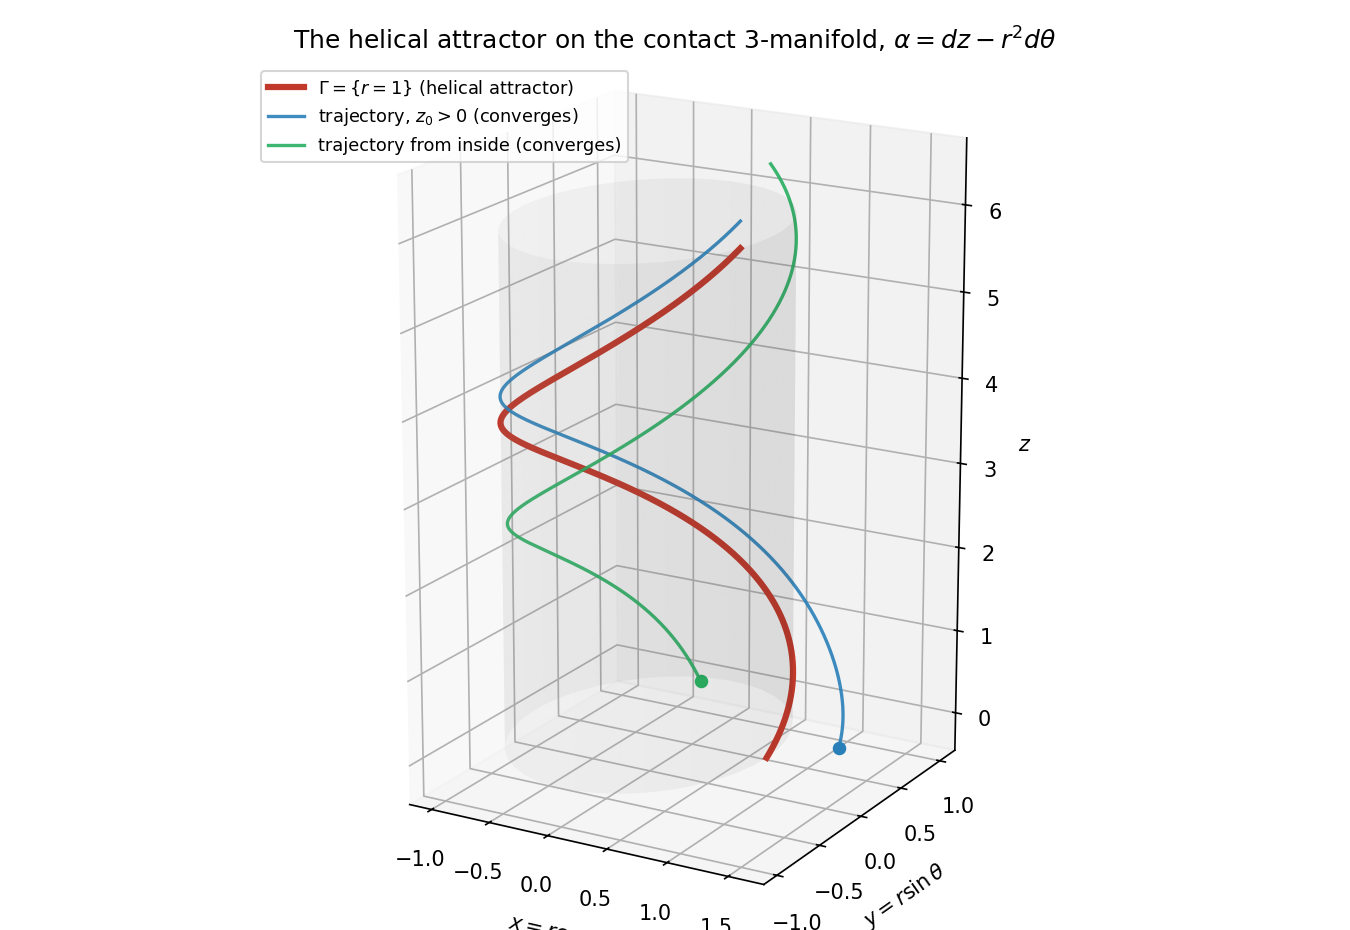
\includegraphics[width=0.78\textwidth]{fig1_helix3d.png}
\caption{The helical attractor $\Gam=\{r=1\}$ (red) on the contact manifold,
with two trajectories of~\eqref{eq:model} (cubic closure) started off the
cylinder at $z_0>0$ and converging onto it. The transverse coordinate is
$r$; the flow advances uniformly in $\theta$ and $z$.}
\label{fig:helix3d}
\end{figure}

Set $\eps:=r-1$. Linearising~\eqref{eq:model} about $\Gam$ using
\eqref{eq:closure-cond} gives the \emph{transverse linear equation}
\begin{equation}\label{eq:lin}
\dot\eps \;=\; f'(1)\,(1-e^{-z})\,\eps \;=\; 2\,\eps\,(e^{-z}-1),
\qquad z=z_0+t,
\end{equation}
which is independent of the closure. All near--helix statements
(\S\S\ref{sec:exponent}--\ref{sec:neutral}) follow from~\eqref{eq:lin}; the
closure enters only in the global statements of \S\ref{sec:closure}.

\section{Closed form and the preserved exponent}\label{sec:exponent}

\begin{theorem}[Closed form; invariance of the exponent]\label{thm:exponent}
The solution of~\eqref{eq:lin} with $z=z_0+t$ is
\begin{equation}\label{eq:closedform}
\eps(t)\;=\;\eps_0\,\exp\!\Bigl(-2t + 2e^{-z_0}\bigl(1-e^{-t}\bigr)\Bigr).
\end{equation}
Consequently, for $\eps_0\neq0$,
\begin{equation}
\mu \;:=\; \lim_{t\to\infty}\frac1t\,\ln\frac{|\eps(t)|}{|\eps_0|}
\;=\; -2 .
\end{equation}
\end{theorem}

\begin{proof}
Separating variables in~\eqref{eq:lin},
$\dd(\ln|\eps|) = 2(e^{-(z_0+t)}-1)\dd t$, and integrating,
\[
\ln|\eps(t)|-\ln|\eps_0|
= 2\!\int_0^t\!\bigl(e^{-(z_0+s)}-1\bigr)\dd s
= 2\bigl(-e^{-(z_0+t)}+e^{-z_0}\bigr)-2t
= -2t + 2e^{-z_0}(1-e^{-t}),
\]
which is~\eqref{eq:closedform}. The bracketed term is bounded by $2e^{-z_0}$
uniformly in $t$, so
$\frac1t\ln|\eps/\eps_0| = -2 + \tfrac{2e^{-z_0}(1-e^{-t})}{t}\to-2$.
\end{proof}

\begin{remark}[Why the modulation is invisible to the exponent]
Because $z$ advances linearly, $\int_0^\infty e^{-(z_0+s)}\dd s=e^{-z_0}<\infty$:
the $e^{-z}$ term is \emph{integrable along the flow}. It therefore shifts
$\ln|\eps|$ by a bounded amount and can never alter the asymptotic rate. The
verified constant $\mu=-2$ survives the new ingredient untouched; only the
transient is reshaped.
\end{remark}

\section{The neutral line \texorpdfstring{$z=0$}{z=0}}\label{sec:neutral}

\begin{theorem}[Sign of the instantaneous rate]\label{thm:neutral}
Let $\rho(z):=2(e^{-z}-1)$ be the instantaneous transverse rate,
$\frac{\dd}{\dd t}\ln|\eps| = \rho(z)$. Then
\[
\rho(z)>0\ (z<0),\qquad \rho(0)=0,\qquad \rho(z)<0\ (z>0).
\]
The locus $z=0$ is non--hyperbolic (loss of transverse hyperbolicity), and for
$z<0$ the transverse flow is the exact time reversal of the $z>0$ flow.
\end{theorem}

\begin{proof}
$\rho$ has the sign of $e^{-z}-1$, hence of $-z$; it vanishes only at $z=0$.
Writing $\dot\eps=\lambda(z)f_1(\eps)$ with $\lambda(z)=1-e^{-z}$ and
$f_1(\eps)=-2\eps+O(\eps^2)$, the factor $\lambda$ changes sign at $z=0$, and
$\lambda(-z')=-\,\lambda(z')\,e^{-z'}$ shows the two half--line flows are
related by time reversal up to the positive reparametrisation $e^{-z'}$.
\end{proof}

\noindent The two half--lines and the neutral locus are summarised in the
regime diagram, Fig.~\ref{fig:regime}.

\begin{figure}[t]
\centering
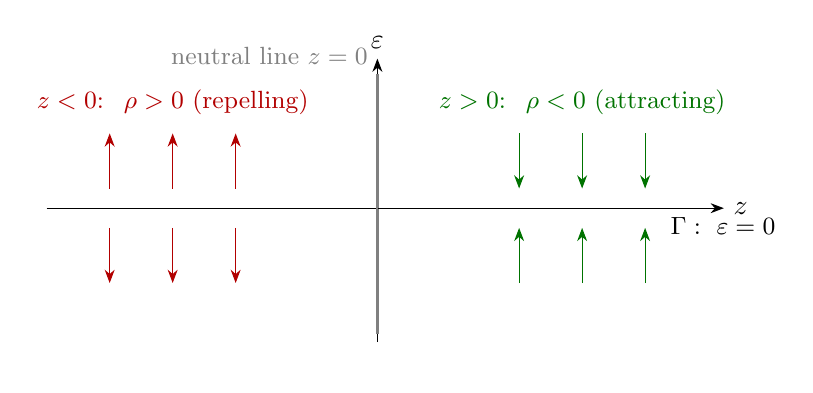
\begin{tikzpicture}[>=Stealth,scale=1.0]
% axes
\draw[->] (-4.2,0)--(4.4,0) node[right]{$z$};
\draw[->] (0,-1.7)--(0,1.9) node[above]{$\eps$};
\node[below] at (0,-1.75) {};
% neutral line
\draw[very thick,gray] (0,-1.6)--(0,1.7);
\node[gray,above left] at (0,1.7) {\small neutral line $z=0$};
% left region: repelling (arrows away from eps=0)
\node[red!70!black] at (-2.6,1.35) {\small $z<0$: \ $\rho>0$ (repelling)};
\foreach \x in {-3.4,-2.6,-1.8} {
  \draw[->,red!70!black] (\x,0.25)--(\x,0.95);
  \draw[->,red!70!black] (\x,-0.25)--(\x,-0.95);
}
% right region: attracting (arrows toward eps=0)
\node[green!45!black] at (2.6,1.35) {\small $z>0$: \ $\rho<0$ (attracting)};
\foreach \x in {1.8,2.6,3.4} {
  \draw[->,green!45!black] (\x,0.95)--(\x,0.25);
  \draw[->,green!45!black] (\x,-0.95)--(\x,-0.25);
}
% helix line eps=0
\draw[dashed] (-4,0)--(4.2,0);
\node[below right] at (3.6,0) {\small $\Gam:\ \eps=0$};
\end{tikzpicture}
\caption{Transverse regime diagram in the $(z,\eps)$ plane. The helix
$\eps=0$ is transversally attracting for $z>0$ and repelling for $z<0$;
$z=0$ is the non--hyperbolic neutral line. Every trajectory sweeps
$z=z_0+t$ rightward at unit rate, so it undergoes a \emph{slow passage}
through this stability reversal.}
\label{fig:regime}
\end{figure}

\begin{remark}[Swept (dynamic) bifurcation]
Since every orbit carries its own control parameter $z$ through the reversal
at unit rate, the transient ``grow while $z<0$, decay while $z>0$'' is the
canonical signature of \emph{slow passage through a bifurcation}
\cite{Kuznetsov}. This is the correct technical home for the ``eye''--like
transient concentration near $\Gam$: not a static bifurcation of a phase
portrait, but a swept passage through a stability--reversal surface.
\end{remark}

\section{Closure dependence: the escape basin}\label{sec:closure}

Theorems~\ref{thm:exponent}--\ref{thm:neutral} are closure--free. The
\emph{global} fate is not.

\begin{theorem}[Finite--time escape for super--linear closures]\label{thm:escape}
For the cubic closure $f_{\mathrm{cub}}(r)=r-r^3$ and $r_0>1$, there is a
threshold $z_0^\ast(\eps_0)$ such that any trajectory with $z_0<z_0^\ast(\eps_0)$
blows up in finite time, escaping to $r=\infty$ while still in the region
$z<0$. Empirically (bisection at \texttt{rtol}$=10^{-10}$),
\begin{equation}\label{eq:boundary}
z_0^\ast(\eps_0)\;\approx\;-\ln\!\Bigl[\tfrac{-\ln\eps_0 + C}{2}\Bigr],
\qquad C\approx 3.68,
\end{equation}
with $z_0^\ast(0.01)\approx-1.495$ (blow--up at $t\approx0.38$).
\end{theorem}

\noindent The double--logarithmic form of~\eqref{eq:boundary} is not fitted
noise: escape occurs when the linear transient amplification
$\eps_0\exp(2e^{-z_0})$ first reaches $O(1)$ --- i.e.\ when
$\ln\eps_0+2e^{-z_0}\sim\text{const}$ --- which inverts precisely
to~\eqref{eq:boundary}. Thus the near--helix linear analysis
\emph{predicts its own basin boundary}, with the nonlinearity fixing only the
$O(1)$ threshold. Figures~\ref{fig:split}--\ref{fig:basin} display the split
and the boundary curve.

\begin{proposition}[Global attraction for bounded closures]\label{prop:bounded}
If $f$ is bounded and satisfies~\eqref{eq:closure-cond}, then no trajectory of
\eqref{eq:model} with $r_0>0$ escapes in finite time, and every such
trajectory satisfies $r(t)\to1$.
\end{proposition}

\begin{proof}
Boundedness gives $|\dot r|\le \|f\|_\infty|1-e^{-z}|\le\|f\|_\infty$, so $r$
grows at most linearly and remains finite for all finite $t$: no blow--up.
Since $z=z_0+t\to+\infty$, eventually $1-e^{-z}>0$; on that region
\eqref{eq:closure-cond} gives $\dot r=f(r)(1-e^{-z})$ with $f(r)(r-1)<0$, so
$r=1$ is globally attracting in $r>0$ and $r(t)\to1$.
\end{proof}

\begin{corollary}
``Where the flow fails to converge'' is a genuine, sharply predictable
prediction \emph{iff} the closure permits super--linear growth. The bounded
closure~$f_{\mathrm{sat}}$ realises global attraction with the identical
linearisation~\eqref{eq:lin}; e.g.\ at $z_0=-5,\ \eps_0=0.01$ it drifts to
$r_{\max}\approx24.5$ and returns to $|\eps|\sim10^{-15}$. The linearisation
alone does not determine which case obtains.
\end{corollary}

\begin{figure}[t]
\centering
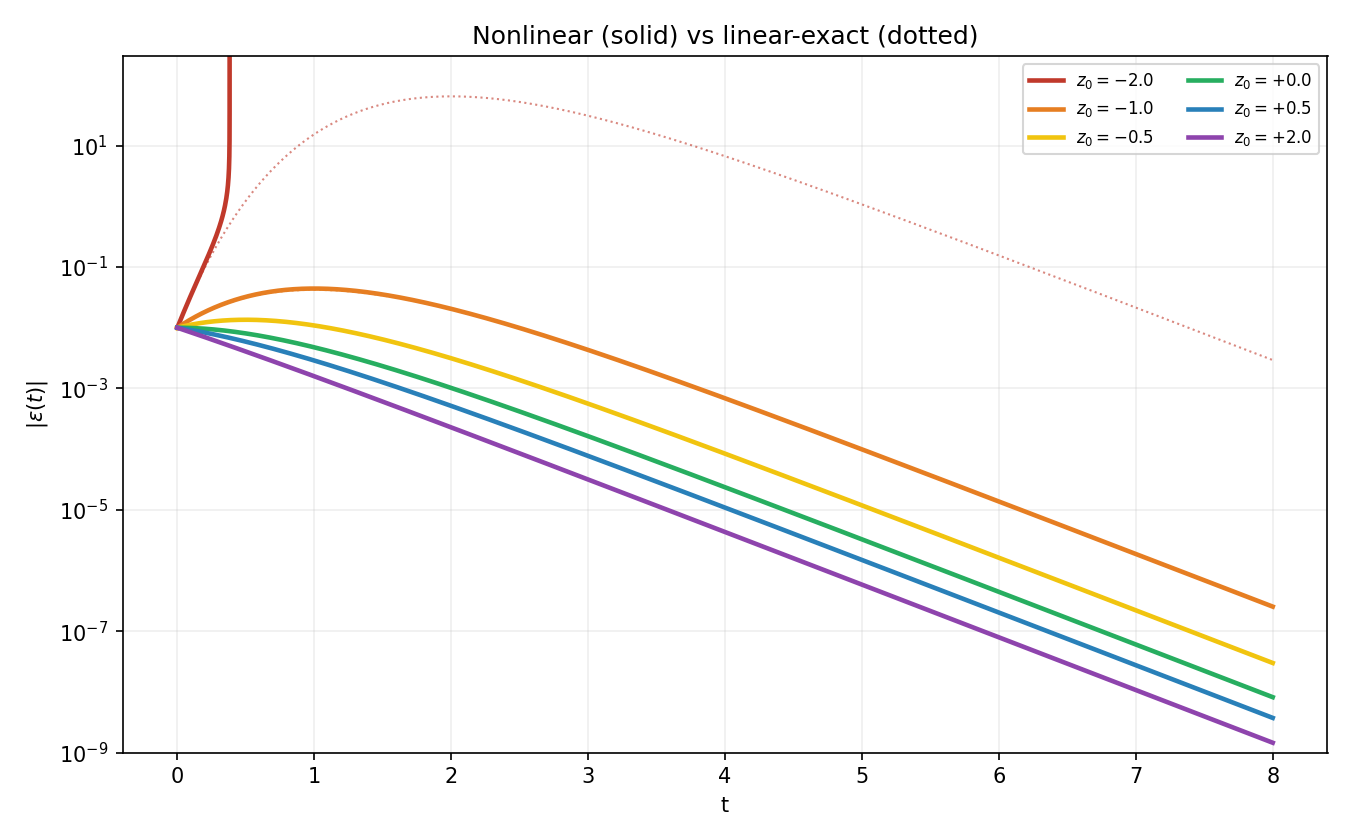
\includegraphics[width=0.86\textwidth]{helix_split.png}
\caption{Cubic closure, $r_0=1.01$. Solid: nonlinear $|\eps(t)|$; dotted:
the exact linear prediction~\eqref{eq:closedform}. For $z_0\gtrsim z_0^\ast$
all curves decay at slope $-2$ (the exponent of Thm.~\ref{thm:exponent}). The
$z_0=-2$ curve escapes at $t\approx0.38$: a finite--time event the
\emph{linear} model structurally cannot exhibit.}
\label{fig:split}
\end{figure}

\begin{figure}[t]
\centering
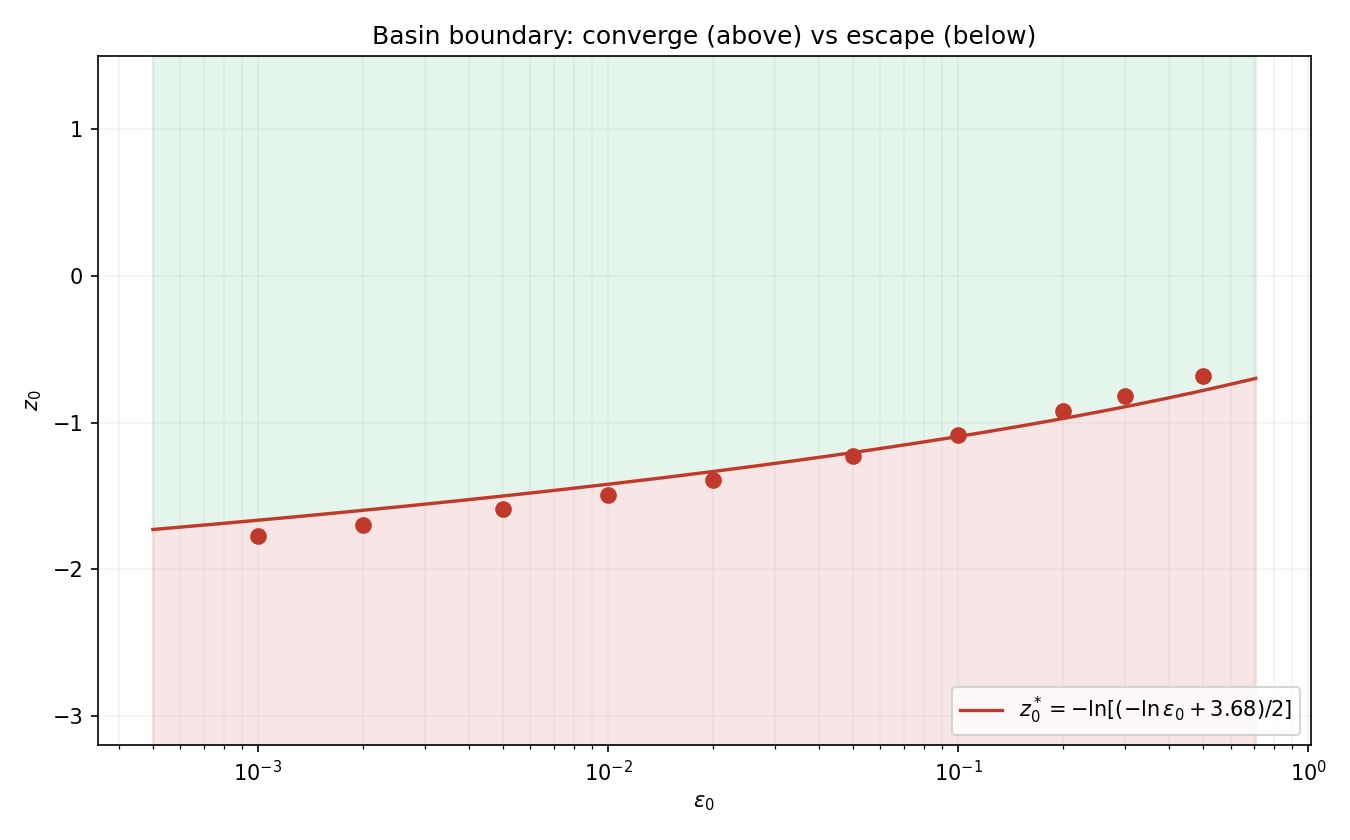
\includegraphics[width=0.80\textwidth]{basin_boundary.png}
\caption{Basin boundary in the $(\eps_0,z_0)$ plane. Points: numerically
located escape threshold for the cubic closure; curve: the double--log
fit~\eqref{eq:boundary}. Above the curve, trajectories converge; below, they
escape in finite time. The bounded (saturating) closure has \emph{no} such
boundary --- it converges everywhere.}
\label{fig:basin}
\end{figure}

\section{Bifurcation structure: a degenerate Hopf}\label{sec:hopf}

The events of \S\ref{sec:neutral} concern the \emph{real} transverse eigenvalue
of the existing cycle. A distinct, genuinely Hopf event lives at the axis.

\begin{theorem}[Degenerate Hopf at $r=0$]\label{thm:hopf}
In Cartesian coordinates $(x,y)=(r\cos\theta,r\sin\theta)$ with
$\dot\theta=\omega$, the linearisation of~\eqref{eq:model} at the axis
equilibrium $r=0$ is
\[
J(0)=\begin{pmatrix}\lambda(z)&-\omega\\ \omega&\lambda(z)\end{pmatrix},
\qquad \lambda(z)=1-e^{-z},
\]
with eigenvalues $\lambda(z)\pm i\omega$ crossing the imaginary axis
transversally at $z=0$ ($\lambda'(0)=1$). The radial normal form is
$\dot r=\lambda(z)\,r-a(z)\,r^3$ with $a(z)=1-e^{-z}$; hence the first
Lyapunov coefficient $a(z)\to0$ at criticality. The bifurcation is therefore
\emph{degenerate}: the emergent cycle radius is $\sqrt{\lambda/a}\equiv1$,
pinned rather than opening as $\sqrt{\lambda}$.
\end{theorem}

\begin{proof}
Near $r=0$, $\dot r=f(r)(1-e^{-z})=r(1-e^{-z})+O(r^3)$; differentiating
$(x,y)$ gives $J(0)$ as stated, eigenvalues $\lambda\pm i\omega$. The Hopf
transversality and nonzero--frequency conditions hold for $\omega\neq0$. The
cubic term of $f_{\mathrm{cub}}$ supplies $a(z)=1-e^{-z}$, which coincides with
the linear coefficient, so the cycle amplitude $\sqrt{\lambda/a}=1$ for all
$z>0$ and does not emanate continuously from the origin.
\end{proof}

\begin{corollary}[Fork, bifurcation form]
Retaining $\Gam=\{r=1\}$ (constant--radius helix) forces the degenerate Hopf
($a\equiv\lambda$, cycle pre--exists). Demanding a \emph{generic} supercritical
Hopf (fixed $a$, radius $\sqrt{1-e^{-z}}$ born at $z=0$) forces a
$z$--dependent helix radius, breaking the constant helix. The two are mutually
exclusive; see Fig.~\ref{fig:hopf}.
\end{corollary}

\begin{figure}[t]
\centering
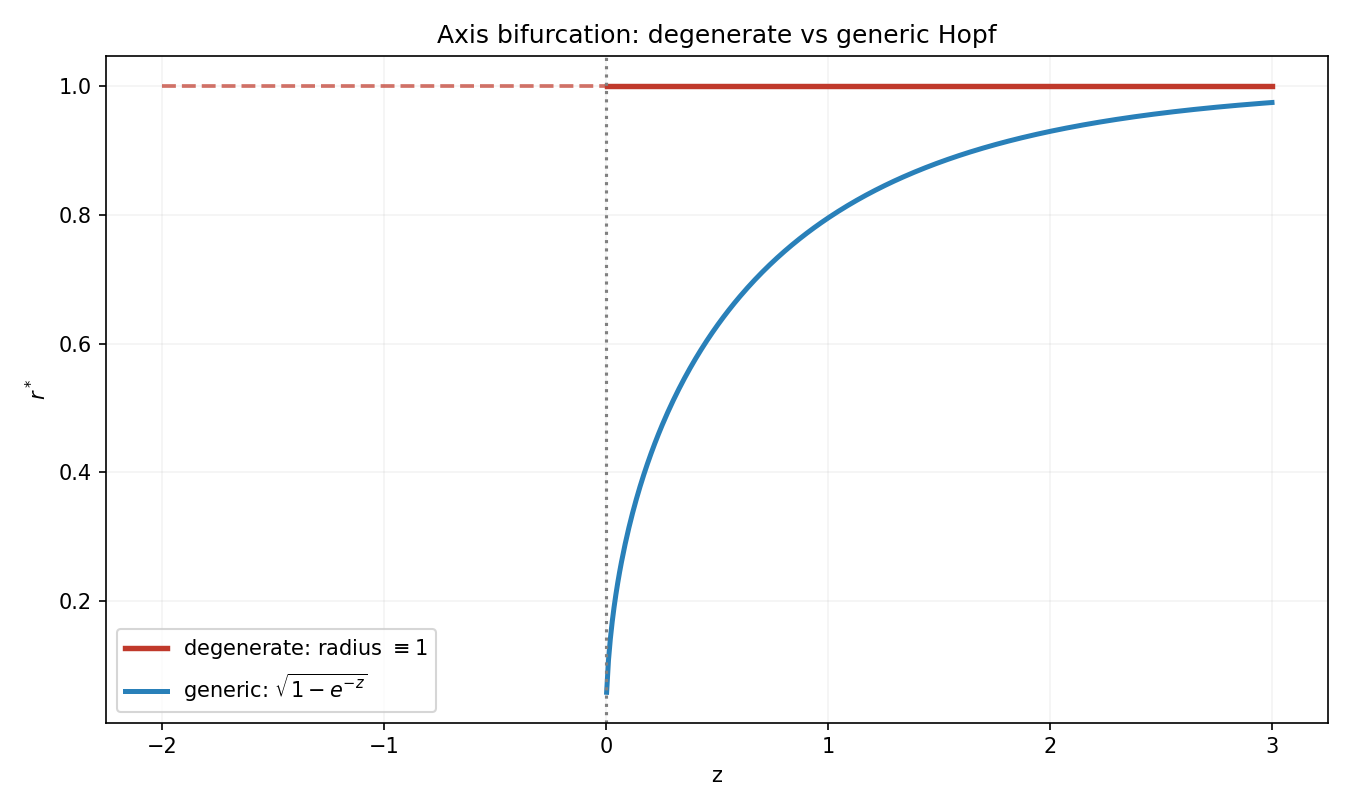
\includegraphics[width=0.82\textwidth]{hopf_diagram.png}
\caption{Bifurcation diagram at the axis. Pinned branch (red): the framework's
degenerate Hopf, radius $\equiv1$, first Lyapunov coefficient vanishing at
$z=0$. Parabolic branch (blue): the generic supercritical Hopf,
$r^\ast=\sqrt{1-e^{-z}}$, which breaks the constant--radius helix.}
\label{fig:hopf}
\end{figure}

\section{A cosmological correspondence and its limits}\label{sec:cosmo}

The $z$--axis admits a clean \emph{kinematic} correspondence, which we state
carefully and then bound.

\begin{proposition}[Kinematic de~Sitter correspondence]\label{prop:cosmo}
Under the identification $z=\ln a$ (number of $e$--folds, $a$ the scale
factor), $\dot z=\dot a/a=H$ (Hubble rate), so $\dot z=1\Leftrightarrow H=1$
$\Leftrightarrow a=e^{t}$ (de~Sitter); and $e^{-z}=a^{-1}\propto T\propto
(1+\text{redshift})$. Moreover the standard Friedmann rate in $e$--folds,
$H(z)=H_0\sqrt{\Omega_\Lambda+\Omega_m e^{-3z}+\Omega_r e^{-4z}}$, and the
model's normalised attraction $1-e^{-z}$ share the same asymptotic structure:
a constant de~Sitter attractor dressed with corrections that decay
exponentially in $e$--folds (Fig.~\ref{fig:cosmo}).
\end{proposition}

This correspondence is \emph{kinematic}, not a derivation. Three obstructions
prevent its promotion to a dynamical model:
\begin{enumerate}[label=(O\arabic*),leftmargin=3em]
\item \textbf{Incomplete dictionary.} Only $z$ is interpreted; $r$ (pinned at
$1$, non--expanding) and $\theta$ have no cosmological meaning. The expanding
coordinate is $z$ alone.
\item \textbf{Asymptotic only.} Constant $H$ is the $\Omega_\Lambda=1$ future
limit; it has no matter or radiation era and hence contradicts the securely
measured decelerating epochs (nucleosynthesis, the acoustic peaks). A realistic
history needs $\dot z=H(z)$ \emph{varying}.
\item \textbf{Wrong power.} The correction $e^{-z}=a^{-1}$ corresponds to
equation of state $w=-\tfrac23$ (a frustrated--network component), not to
matter $a^{-3}$ or radiation $a^{-4}$.
\end{enumerate}

\begin{figure}[t]
\centering
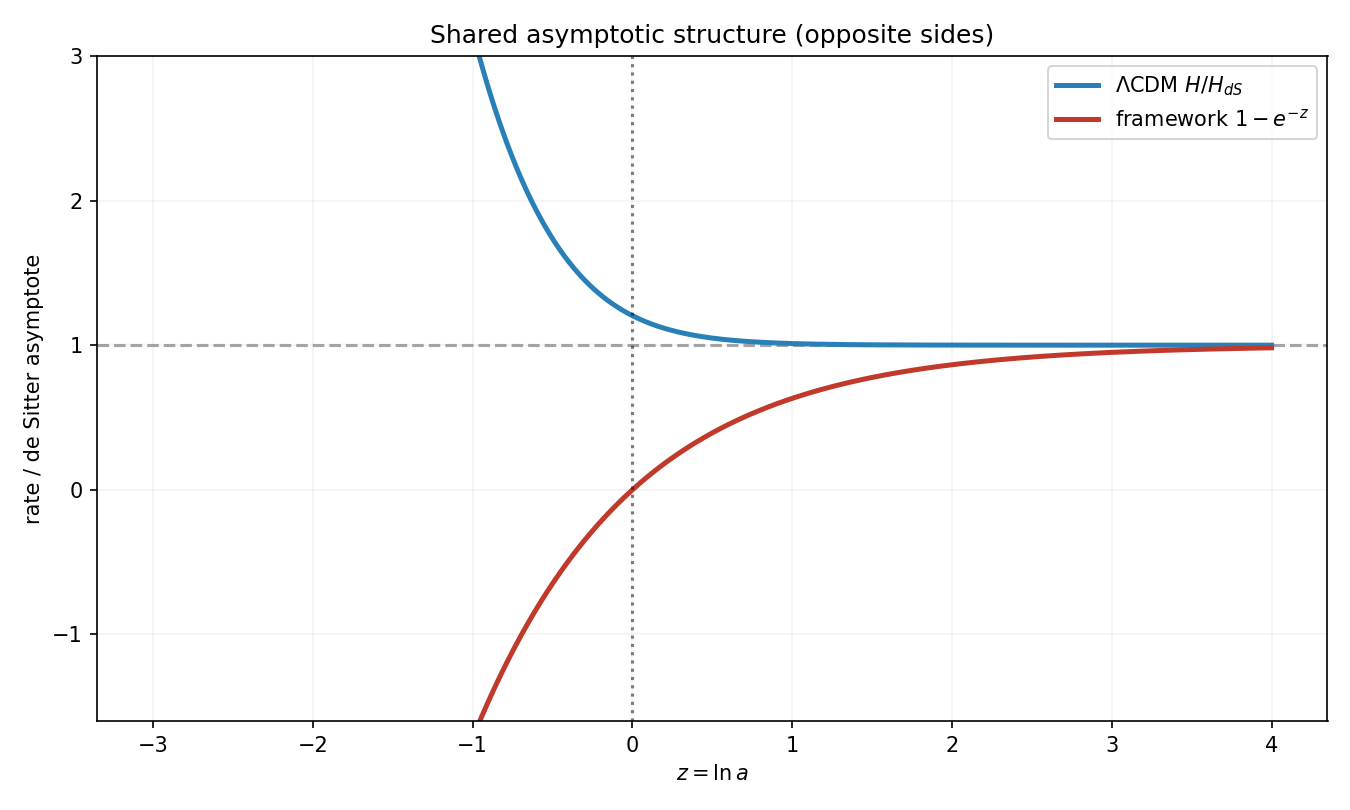
\includegraphics[width=0.82\textwidth]{cosmo_parallel.png}
\caption{Shared asymptotic structure. $\Lambda$CDM approaches the de~Sitter
attractor from above (early universe expands faster); the model's attraction
approaches it from below (early attraction weaker, repelling for $z<0$). Same
asymptote; opposite--signed, different--power corrections. Coincidence of the
two would be spurious; the honest statement is structural analogy.}
\label{fig:cosmo}
\end{figure}

\section{A contact--Hamiltonian no--go}\label{sec:nogo}

We ask whether the geometry \emph{forces} an expansion law $H(z)$, promoting
$\dot z=1$ to $\dot z=H(z)$. The contact Hamilton equations for
$\mathcal H(\theta,p,z)$ with $\alpha=\dd z-p\,\dd\theta$ read
\cite{BravettiCruzTapias}
\begin{equation}\label{eq:contactHamEq}
\dot\theta=\partial_p\mathcal H,\qquad
\dot p=-\bigl(\partial_\theta\mathcal H + p\,\partial_z\mathcal H\bigr),\qquad
\dot z=p\,\partial_p\mathcal H-\mathcal H .
\end{equation}

\begin{theorem}[No coexistence of attractor and de~Sitter rate]\label{thm:nogo}
Consider~\eqref{eq:contactHamEq} with constant rotation $\dot\theta\equiv1$.
\begin{enumerate}[label=(\alph*),leftmargin=2.4em]
\item Then $\mathcal H=p+g(\theta,z)$ for some $g$, and consequently $\dot p$ is
affine in $p$: it contains no $p^2$ term. The cubic limit cycle
($\dot p\ni-2p^2(1-e^{-z})$) is therefore \emph{not} generated by any such
contact Hamiltonian.
\item In the $\theta$--independent linear reduction $g=g(z)$, the expansion
rate and transverse rate are $H(z):=\dot z=-g(z)$ and $c(z)=-g'(z)$, so
\begin{equation}\label{eq:locking}
c(z)\;=\;H'(z)\qquad\text{(locking identity).}
\end{equation}
\item Hence if $c(z)\to-2$ (a transverse attractor, matching $\mu_{\max}$),
then $H(z)=H(z_0)+\int_{z_0}^{z}c\to-\infty$: the expansion rate is unbounded
below and cannot converge to a positive constant. A transverse contact
attractor and a de~Sitter expansion rate are mutually exclusive on
$(\,M,\alpha\,)$.
\end{enumerate}
\end{theorem}

\begin{proof}
(a) $\partial_p\mathcal H=\dot\theta=1$ forces $\mathcal H=p+g(\theta,z)$.
Then $\dot p=-\partial_\theta g-p\,\partial_z g$, affine in $p$; a $p^2$
term is impossible. (b) With $g=g(z)$: $\dot z=p\cdot1-(p+g)=-g(z)=:H(z)$ and
$\dot p=-g'(z)\,p$, i.e.\ $c(z)=-g'(z)=H'(z)$. (c) Integrate~\eqref{eq:locking}:
$H(z)-H(z_0)=\int_{z_0}^z c$. If $c\to-2$ the integral diverges to $-\infty$,
so $H\to-\infty$; in particular $H\not\to L$ for any finite $L>0$.
\end{proof}

\begin{remark}
Every contact--structure--preserving flow \emph{is} a contact Hamiltonian flow;
thus Theorem~\ref{thm:nogo}(a) says the stated dynamics, under constant
rotation, do not preserve the advertised contact structure --- the form
$\alpha$ is, with respect to the flow, decorative unless $\dot\theta$ is allowed
to vary with $r$. The single available escape (variable rotation
$\dot\theta=\omega(r)$) relaxes~\eqref{eq:closure-cond}'s constant period to a
cycle--only statement and owes its own derivation.
\end{remark}

\section{Discussion}\label{sec:discussion}

The model is a faithful \emph{relaxation} system: a dissipative flow whose
transverse contraction ($\mu=-2$) and whose $z$--advance are, under the contact
structure, rigidly coupled through~\eqref{eq:locking}. That coupling is exactly
what makes it a poor \emph{expansion} model --- Theorem~\ref{thm:nogo} is a
structural obstruction, not a gap to be closed. The productive readings are
therefore (i) the swept--bifurcation transient of \S\ref{sec:neutral}, (ii) the
closure--diagnostic of \S\ref{sec:closure} (super--linear vs.\ bounded decides
global fate), and (iii) the degenerate Hopf of \S\ref{sec:hopf} as a
non--generic normal form worth cataloguing. The cosmological correspondence of
\S\ref{sec:cosmo} is genuine but strictly kinematic; its three obstructions and
the no--go together delimit precisely what the geometry can and cannot claim.

\appendix
\section{Exercises}\label{sec:exercises}

\begin{exercise}[Closed form]
Verify by direct differentiation that~\eqref{eq:closedform} solves
\eqref{eq:lin}. \emph{Hint:} compute $\frac{\dd}{\dd t}\ln|\eps|$.
\end{exercise}

\begin{exercise}[Exponent]
From~\eqref{eq:closedform}, show $\mu=-2$ and identify the exact bounded
correction to $\ln|\eps|$. Explain, in one sentence, why an $e^{-z}$ term with
$z$ growing \emph{sub}linearly (say $z=\sqrt t$) would \emph{not} leave $\mu$
invariant.
\end{exercise}

\begin{exercise}[Transient peak]
For $z_0<0$ show the transient $|\eps|$ peaks at $z=0$ (i.e.\ $t=-z_0$) with
amplification $|\eps(t^\ast)|/|\eps_0|=\exp\!\bigl(2e^{-z_0}-2|z_0|-2\bigr)$,
and give its leading behaviour as $z_0\to-\infty$.
\end{exercise}

\begin{exercise}[Neutral line]
Prove Theorem~\ref{thm:neutral}. Why is $z=0$ \emph{not} a saddle--node,
transcritical, or pitchfork bifurcation of~\eqref{eq:model}? \emph{Hint:}
examine what the whole vector field does at $z=0$.
\end{exercise}

\begin{exercise}[Finite--time escape]
For the cubic closure freeze $z<0$ so that $1-e^{-z}=:-\kappa<0$. Show
$\dot r=-\kappa(r-r^3)$ has solutions leaving every bounded set in finite time
for $r_0>1$, and estimate the blow--up time. Explain why the swept problem
($z=z_0+t$) escapes only when $z_0$ is sufficiently negative.
\end{exercise}

\begin{exercise}[Global attraction]
Prove Proposition~\ref{prop:bounded}. Where exactly does boundedness of $f$
enter, and where does condition~\eqref{eq:closure-cond} enter?
\end{exercise}

\begin{exercise}[Hopf eigenvalues]
Derive $J(0)$ in Theorem~\ref{thm:hopf} and its eigenvalues. Verify the Hopf
transversality condition and state where nonzero frequency is used.
\end{exercise}

\begin{exercise}[Generic vs.\ degenerate]
For $\dot r=\lambda r-a r^3$ with \emph{constant} $a>0$, show the stable cycle
radius is $\sqrt{\lambda/a}$. Contrast with $a=\lambda=1-e^{-z}$ and explain in
one sentence why the framework's helix has fixed radius.
\end{exercise}

\begin{exercise}[Cosmological kinematics]
Show $z=\ln a\Rightarrow\dot z=H$. Identify the de~Sitter case and compute the
equation of state $w$ for which $\rho\propto a^{-1}$ (i.e.\ the ``power'' of the
$e^{-z}$ correction). Which standard component, if any, does it match?
\end{exercise}

\begin{exercise}[Contact no--go]
Starting from~\eqref{eq:contactHamEq}, impose $\dot\theta\equiv1$ and derive
$\mathcal H=p+g(\theta,z)$. Prove the locking identity~\eqref{eq:locking} in the
$\theta$--independent case and deduce Theorem~\ref{thm:nogo}(c). Finally,
sketch how a variable rotation $\dot\theta=\omega(r)$ evades part~(a).
\end{exercise}

\section{Solutions (sketches)}\label{sec:solutions}

\noindent\textbf{1.} $\frac{\dd}{\dd t}\ln|\eps|=-2+2e^{-z_0}\!\cdot e^{-t}
=2(e^{-(z_0+t)}-1)$, matching~\eqref{eq:lin}.\\[2pt]
\textbf{2.} $\ln|\eps/\eps_0|=-2t+2e^{-z_0}(1-e^{-t})$; the bounded correction
is $2e^{-z_0}(1-e^{-t})\to2e^{-z_0}$, so $\mu=-2$. With $z=\sqrt t$,
$\int^\infty e^{-\sqrt s}\dd s=\infty$ diverges more slowly than $t$ but the
rate term $-1$ is unaffected; the point is that any $\int_0^t e^{-z(s)}\dd s$
growing linearly in $t$ \emph{would} shift $\mu$ --- integrability is what
protects it. (For $z=\sqrt t$, $\tfrac1t\int_0^t e^{-\sqrt s}\dd s\to0$, so
$\mu=-2$ still; the invariance fails only if $e^{-z}$ has nonzero Ces\`aro
mean, e.g.\ $z$ bounded.)\\[2pt]
\textbf{3.} $\ln|\eps|$ is maximised where $\rho(z)=0$, i.e.\ $z=0$, $t=-z_0$.
Substitute into~\eqref{eq:closedform}: exponent
$-2(-z_0)+2e^{-z_0}(1-e^{z_0})=2z_0+2e^{-z_0}-2$; hence amplification
$\exp(2e^{-z_0}-2|z_0|-2)$ (using $|z_0|=-z_0$). As $z_0\to-\infty$ it grows
like $\exp(2e^{|z_0|})$.\\[2pt]
\textbf{4.} Sign of $\rho$ is that of $-z$; $z=0$ is the unique zero and
$\rho'(0)=-2\neq0$ for the \emph{rate}, but the full field
$\dot r=f(r)(1-e^{-z})$ vanishes identically at $z=0$ (every $r$ is
momentarily fixed), so no fixed point is created, destroyed, or exchanged ---
disqualifying the codimension--one normal forms. It is a neutral
stability--reversal locus.\\[2pt]
\textbf{5.} $\dot r=-\kappa(r-r^3)=\kappa r^3(1-r^{-2})$; for $r_0>1$,
$\dot r>0$ and $\dot r\gtrsim\kappa r^3/2$ for $r\ge\sqrt2$, whose solution
$\sim(r_0^{-2}-\kappa t)^{-1/2}$ blows up by
$t_\ast\lesssim r_0^{-2}/\kappa$. In the swept problem $\kappa=e^{-z}-1$ shrinks
as $z\to0^-$; only sufficiently negative $z_0$ gives a window long/strong enough
to reach blow--up before $z$ crosses $0$.\\[2pt]
\textbf{6.} See Prop.~\ref{prop:bounded}: boundedness prevents finite--time
blow--up (bounds $|\dot r|$); \eqref{eq:closure-cond} gives the sign of $f$ that
makes $r=1$ globally attracting once $1-e^{-z}>0$.\\[2pt]
\textbf{7.} $\dot x=\lambda x-\omega y,\ \dot y=\omega x+\lambda y$ to first
order; eigenvalues $\lambda\pm i\omega$; $\mathrm{Re}=\lambda(z)$,
$\lambda'(0)=e^{0}=1\neq0$ (transversal); $\omega\neq0$ ensures genuine
rotation (nonzero imaginary part).\\[2pt]
\textbf{8.} Setting $\dot r=0$: $r^2=\lambda/a$. For constant $a$,
$r^\ast=\sqrt{\lambda/a}\propto\sqrt\lambda$. For $a=\lambda$,
$r^\ast=1$ independent of $\lambda$: the amplitude decouples from the parameter,
the degenerate case.\\[2pt]
\textbf{9.} $\dot z=\frac{\dd}{\dd t}\ln a=\dot a/a=H$; $H\equiv1\Rightarrow
a=e^t$ (de~Sitter). $\rho\propto a^{-3(1+w)}=a^{-1}\Rightarrow w=-\tfrac23$:
a domain--wall/frustrated--network component, matching neither matter
($w=0$) nor radiation ($w=\tfrac13$).\\[2pt]
\textbf{10.} $\partial_p\mathcal H=1\Rightarrow\mathcal H=p+g(\theta,z)$;
$\theta$--independent $\Rightarrow\dot z=-g$, $\dot p=-g'p$, so
$c=-g'=H'$. If $c\to-2$, $H=\int c\to-\infty$, excluding a positive constant
limit. Variable rotation $\dot\theta=\omega(r)$ makes $\partial_p\mathcal H$
depend on $p$, admitting $p^2$ in $\dot p$ and evading part~(a) --- at the cost
of constant period.

\begin{thebibliography}{9}
\bibitem{Strogatz} S.~H.~Strogatz, \emph{Nonlinear Dynamics and Chaos},
2nd ed., Westview/CRC, 2015.
\bibitem{GuckenheimerHolmes} J.~Guckenheimer and P.~Holmes,
\emph{Nonlinear Oscillations, Dynamical Systems, and Bifurcations of Vector
Fields}, Springer, 1983.
\bibitem{Kuznetsov} Yu.~A.~Kuznetsov, \emph{Elements of Applied Bifurcation
Theory}, 3rd ed., Springer, 2004.
\bibitem{BravettiCruzTapias} A.~Bravetti, H.~Cruz, and D.~Tapias,
\emph{Contact Hamiltonian mechanics}, Annals of Physics \textbf{376} (2017)
17--39.
\bibitem{Weinberg} S.~Weinberg, \emph{Cosmology}, Oxford University Press,
2008.
\bibitem{Mathlib} The mathlib Community, \emph{The Lean mathematical library},
CPP 2020.
\end{thebibliography}

\end{document}
